

\chapter{Analyse des besoins}
Dans l'analyse des besoins on prend compte les nécessités de l'application et du client en analysant les fonctionnalités demandées en établissant un cahier des charges

\section{Cahier des charges}
Un cahier des charges est la première étape dans chaque projet, il
sert à formaliser les besoins et à les expliquer aux différents acteurs pour s’assurer que tout le monde soit d’accord.

\subsection{Identification des acteurs et leurs besoins}
Un acteur, autrement dit utilisateur, est une personne qui engage avec le système, soit d'une façon direct ou indirect.

\begin{enumerate}
	\item \textcolor{red}{Administrateur}: Il est le garant du développement, déroulement  et de l'évolution du site.\\
	Il peut:
	\begin{itemize}
		\item Gérer les comptes des utilisateurs (Ajouter, Modifier, Bloquer, Supprimer).
		\item Gérer les appels d’offres et les soumissions (Ajouter, Modifier, Supprimer).
		\item Gérer les réclamations et les signalements.
	\end{itemize}

	\item \textcolor{red}{Visiteur}: Qui entre sur le site pour la première fois avant d'ouvrir un compte.\\
	Il peut:
	\begin{itemize}
		\item Consulter site  via une application web ou mobile.
		\item S'inscrire dans le site pour devenir un client.
		\item Consulter la liste et les profils des artisans.
	\end{itemize}

	\item \textcolor{red}{Client}: Visiteur ayant un compte.\\
	Il peut:
	\begin{itemize}
		\item Gérer son profil.
		\item Consulter la liste et les profils des artisans.
		\item Poster un appel d’offre.
		\item Gérer ses appels d’offres (Modifier ou Supprimer).
		\item Gérer les soumissions des artisans pour un appel d’offre.
		\item Demander le service d’un artisan.
		\item Évaluer le service d’un artisan.
		\item Signaler un artisan et soumettre une réclamation.
	\end{itemize}

	\item \textcolor{red}{Artisan}: Qui possède un métier, que ce soit maçon, couvreur, plombier, tapissier, chauffagiste, coiffeur, fleuriste, tailleur$\dots$\\
	Il peut:
	\begin{itemize}
		\item Gérer son profile.
		\item Consulter des appels d’offres.
		\item Soumettre des appels d’offres.
		\item Gérer soumissions (Modifier ou Supprimer).
		\item Évaluer un client.
		\item Signaler un client.
	\end{itemize}
\end{enumerate}

\subsection{Besoins non-fonctionnels}
Les besoins non-fonctionnels sont des nécessités non-visible pour l'utilisateur mais sont nécessaires pour avoir une douce expérience dans l'application.\\
\begin{itemize}
\item Le système doit être disponible tout le temps.
\item Le système doit être facile a utiliser.
\item Temps de réponse très court.
\item Les mots de passe sont stockés de manière sécurisée.
\item Le système suffisamment intuitif pour faciliter l’opération au client.
\end{itemize}


\pagebreak
\section{Spécification des besoins}
La spécification des besoins et le premier document produit dans le chapitre d'analyse, elle consiste a décrire les fonctionnalités et leurs contraintes d'une façon simple et lisible a fin de pouvoir les communiquer facilement

\subsection{Diagramme Cas D'utilisation}
Un diagramme de cas d'utilisation nous permet de visualiser les besoins / fonctionnalités de l'application d'une façon abstraite.

\begin{figure}[h!]
\centering
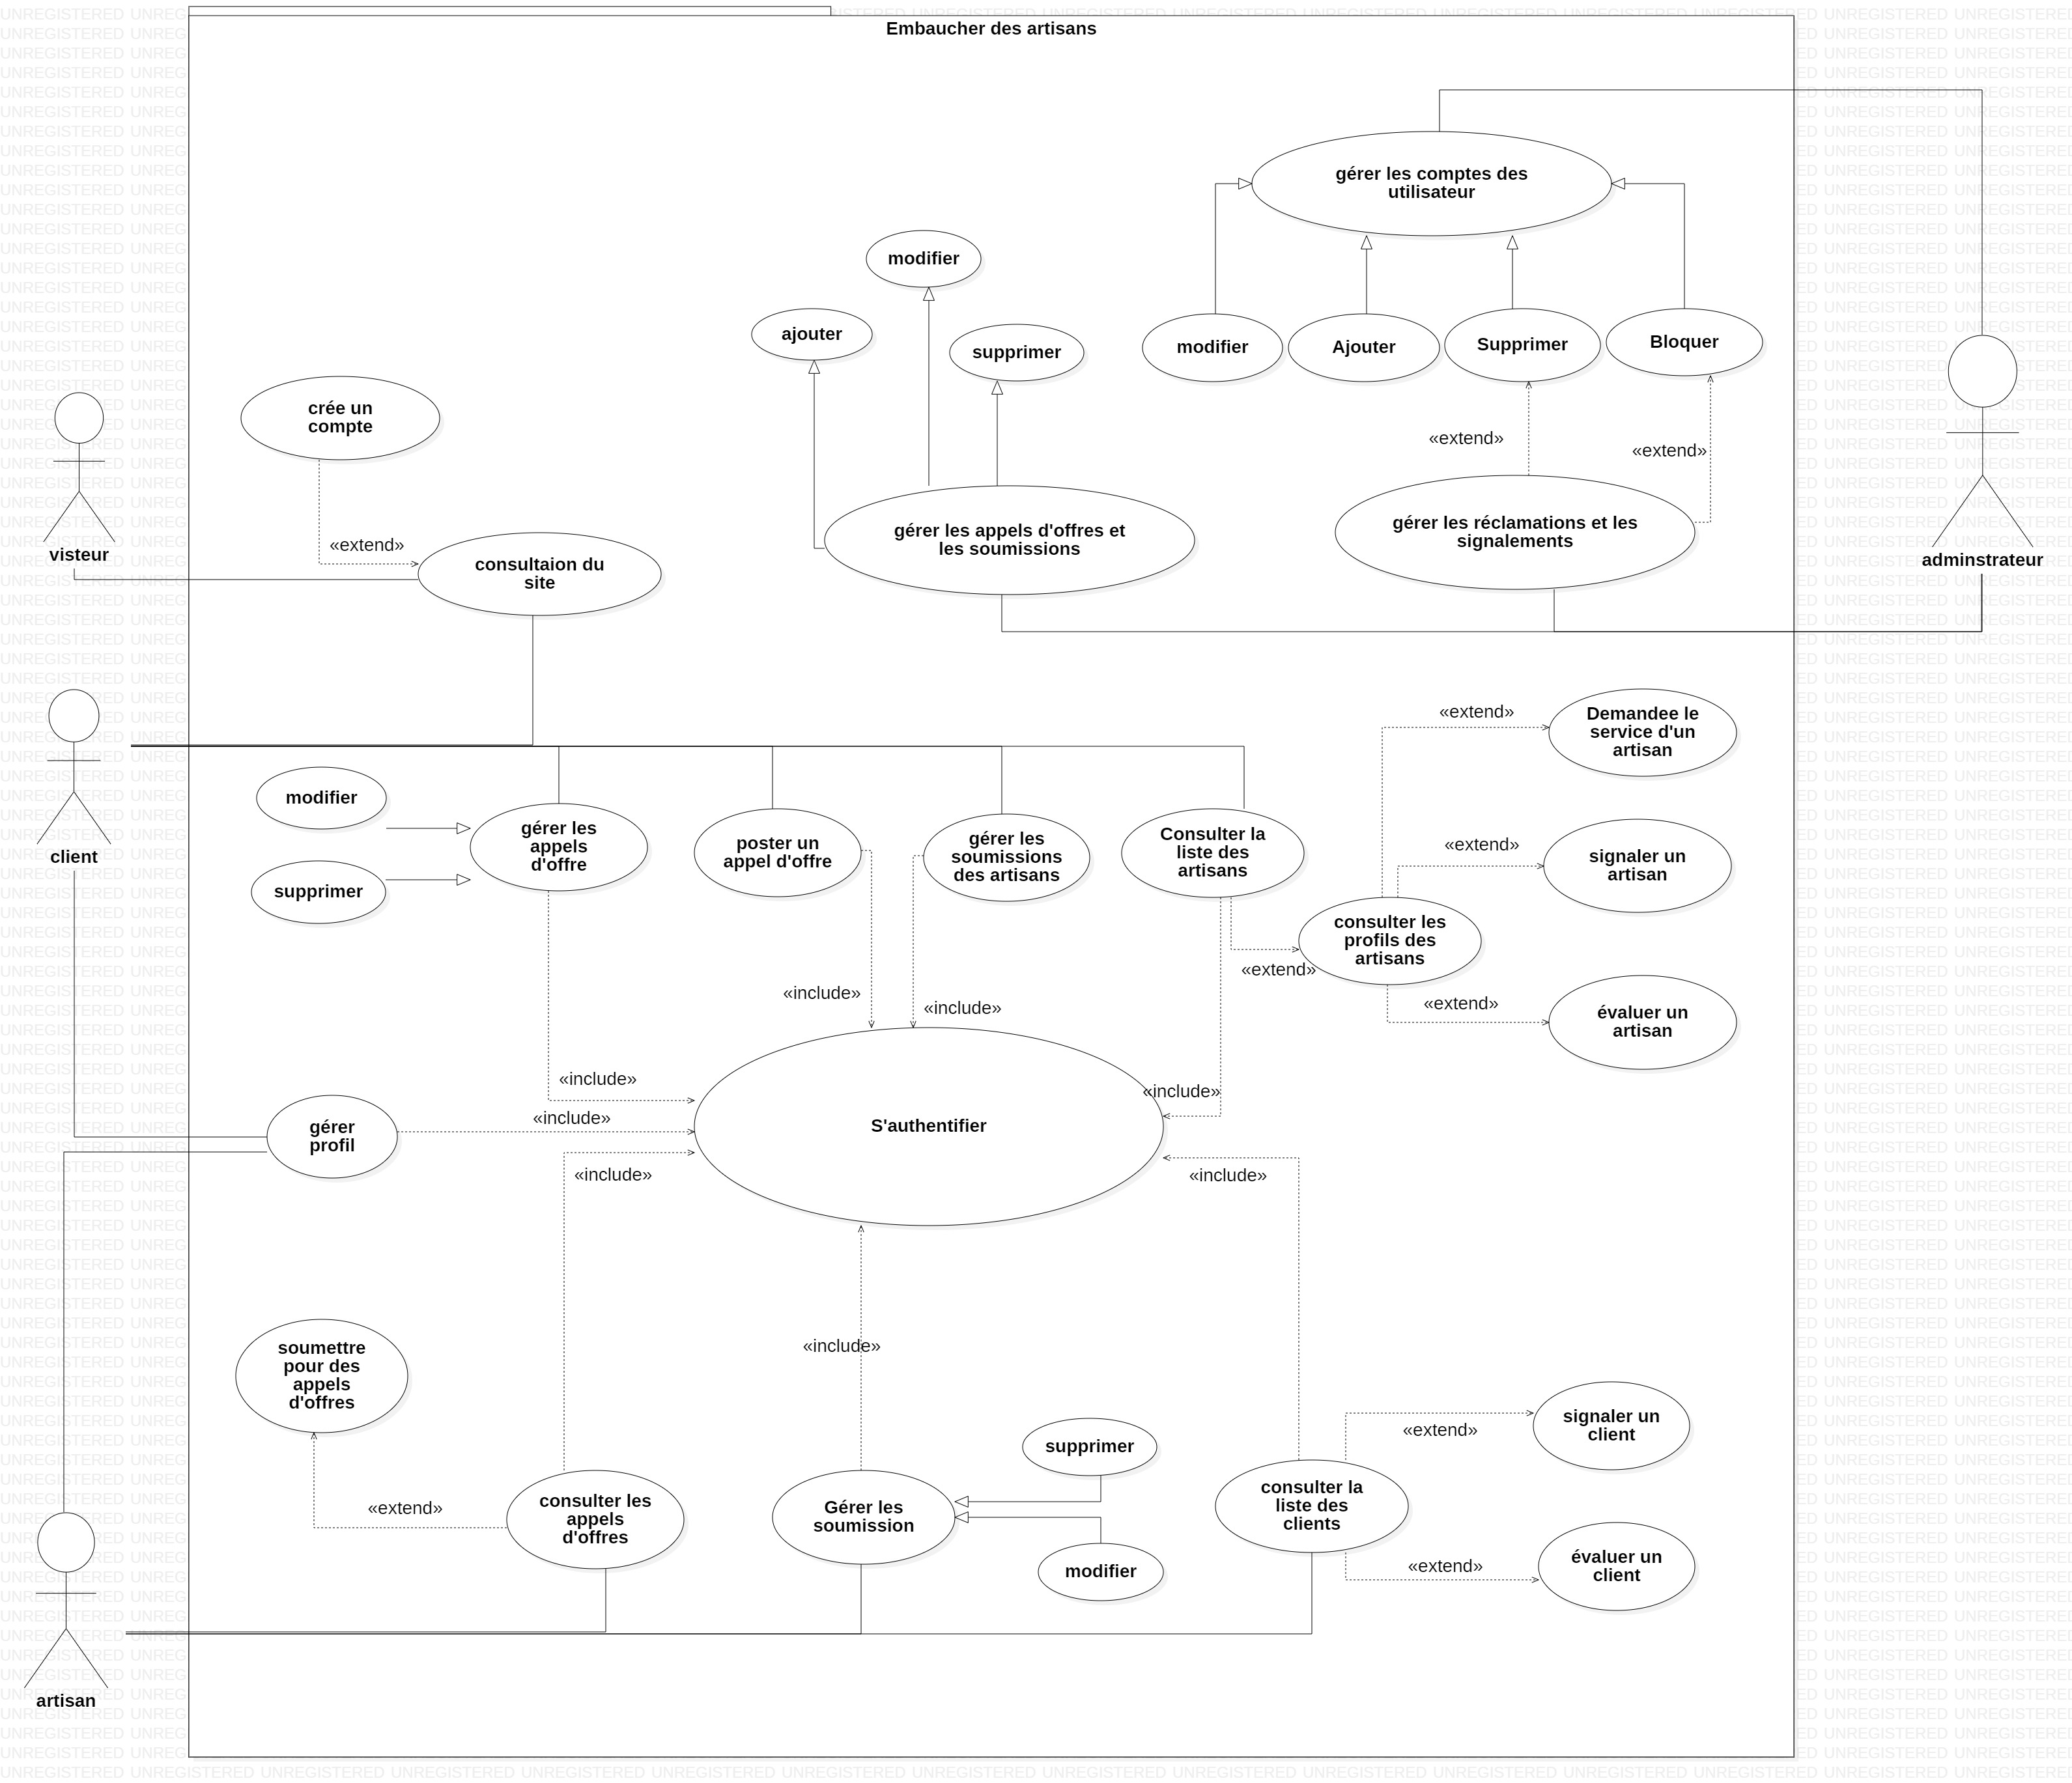
\includegraphics[scale=0.15]{UseCase.jpg}
\caption{Diagramme cas d'utilisation}
\label{fig:use case}
\end{figure}


\section{Descriptions et D.S}
Une description textuelle ou autrement dit fiche descriptive est une autre façon de communiquer les besoins du projet, elle sert à mieux clarifier le cas cité dans le diagramme cas d'utilisation.
Elle cite:\\
 - Un scénario nominal dans laquelle l'exécution se déroule comme prévu sans erreurs.\\
 - Un scénario alternatif dans laquelle l'exécution a eu un problème ou le déroulement a échoué.
 - Un scénario d'erreur ou l'exécution s'arrête complètement.
 
Un diagramme de séquence prend la description textuelle vers un niveau d'abstraction communicable et compréhensible pour mieux clarifier le cas d'utilisation avec la moindre verbosité

\pagebreak
\subsection{Cas d'utilisation Crée compte}
\renewcommand{\arraystretch}{1.3}
\begin{center}
	\begin{table}[H]
			\centering
			\tiny\begin{tabular}{ | l | m{0.51\textheight} |}
			\hline
			\rowcolor[HTML]{06a8ed}
			\textbf{Nom du cas} & Crée un compte \\
			\hline\hline
			\cellcolor[HTML]{99ccff} \textbf{Type} & Principal\\
			\hline
			\cellcolor[HTML]{99ccff} \textbf {Acteur Principal} & Visiteur\\
			\hline
			\cellcolor[HTML]{99ccff} \textbf Objective & Permet à tout visiteur du site de	crée un compte et devenir client\\
			\hline
			\cellcolor[HTML]{99ccff}\textbf {Pré-condition} & Consulter Site\\
			\hline
			\cellcolor[HTML]{99ccff} \textbf {Scénario Nominal} & \parbox{0.43\textheight}{
					\begin{enumerate}
						\vspace{0.01\textheight}
						\item Le visiteur clique << Crée Compte >>.
						\item Le site affiche le formulaire du création des comptes.
						\item Le visiteur remplis les champs affiché.
						\item Le visiteur confirme les informations.
						\item Le système vérifie informations.
						\item Le système crée un compte pour l'utilisateur et le redirige vers son profil.
						\vspace{0.01\textheight}
					\end{enumerate}}\\
			\hline
			\cellcolor[HTML]{99ccff} \textbf {Scénario Alternatif} & \parbox{0.43\textheight}{
				\begin{enumerate}
					\item \textbf{A1: Les informations du visiteur ne sont pas valides:}
						\subitem 5. Le site affiche message d'erreur.\newline						
					La séquence résume du point 2.
					
					\item \textbf{A2: Le compte existe déjà:}
						\subitem 1. Le système demande à l'utilisateur de modifier l'identifiant ou de se connecter\newline
					Le séquence reprend au point 2
				\end{enumerate}}\\
			\hline
			\cellcolor[HTML]{99ccff} \textbf{Scénario d'exception} & --- \\
			\hline
			\cellcolor[HTML]{99ccff} \textbf{Post-condition} & Un nouveau compte client sera crée\\
			\hline
		\end{tabular}
		\caption{Description Crée compte}
		\label{table:create account}
	\end{table}
	\begin{figure}[H]
		\centering
		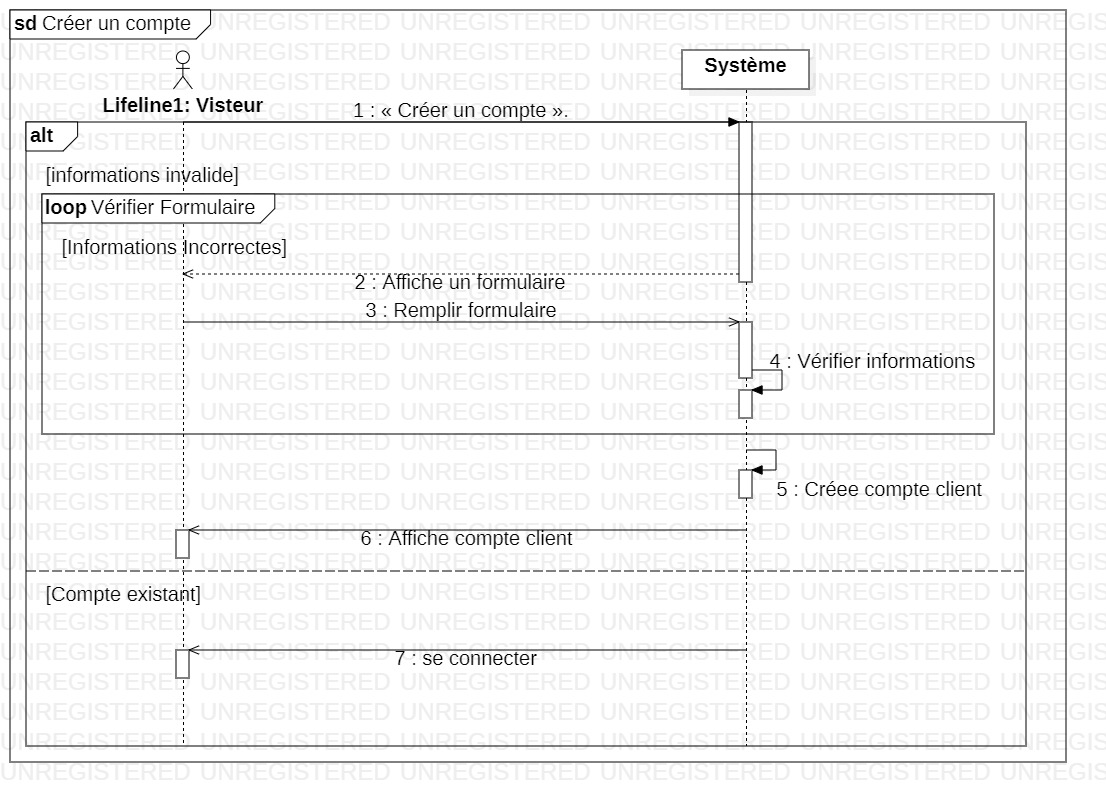
\includegraphics[scale=0.4]{CreateAccount.jpg}
		\caption{Diagramme séquence Crée un compte}
		\label{fig:seq create account}
	\end{figure}
\end{center}


\subsection{Cas d'utilisation Gérer profil (modifier)}
\renewcommand{\arraystretch}{2}
\begin{center}
	\begin{table}[H]
		\centering
		\tiny{\begin{tabular}{ | l | m{0.51\textheight} |}
			\hline
			\rowcolor[HTML]{06a8ed}
									 \textbf{Nom du cas} & Gérer profil (modifier)\\ 
			\hline \hline
			\cellcolor[HTML]{99ccff} \textbf{Type} & Principal\\
			\hline
			\cellcolor[HTML]{99ccff} \textbf{Acteur Principal} & Client, Artisans\\
			\hline
			\cellcolor[HTML]{99ccff} \textbf{Objective} & Permet à l'acteur de modifier les informations de son compte\\
			\hline
			\cellcolor[HTML]{99ccff} \textbf{Pré-condition} & S'authentifier\\
			\hline
			\cellcolor[HTML]{99ccff} \textbf{Scénario Nominal} & \parbox{0.43\textheight}{
					\begin{enumerate}
						\vspace{0.01\textheight}
						\item L'acteur clique << Gérer Profile >>.
						\item Le site affiche toutes informations cecernant l'acteur.
						\item L'acteur peut modifier les informations affichées.
						\item L'acteur confirme les modifications.
						\item Le système vérifie informations.
						\item Le système enregistre les informations.
						\item Le système affiche message de succèss.
						\vspace{0.01\textheight}
					\end{enumerate}}\\
			\hline
			\cellcolor[HTML]{99ccff} \textbf{Scénario Alternatif} & \parbox{0.43\textheight}{
				\begin{enumerate}
					\item \textbf{A1: Les informations de l'acteur ne sont pas valides:}
					\subitem 6. Le site affiche message d'erreur.\newline						
					La séquence résume du point 3.
				\end{enumerate}}\\
			\hline
			\cellcolor[HTML]{99ccff} \textbf{Scénario d'exception} & ---\\
			\hline
			\cellcolor[HTML]{99ccff} \textbf{Post-condition} & La mise-à-jour de profil de l'acteur\\
			\hline
		\end{tabular}}
		\caption{Description Modifier compte}
		\label{table:modifier account}
	\end{table}
	\begin{figure}[H]
		\centering
		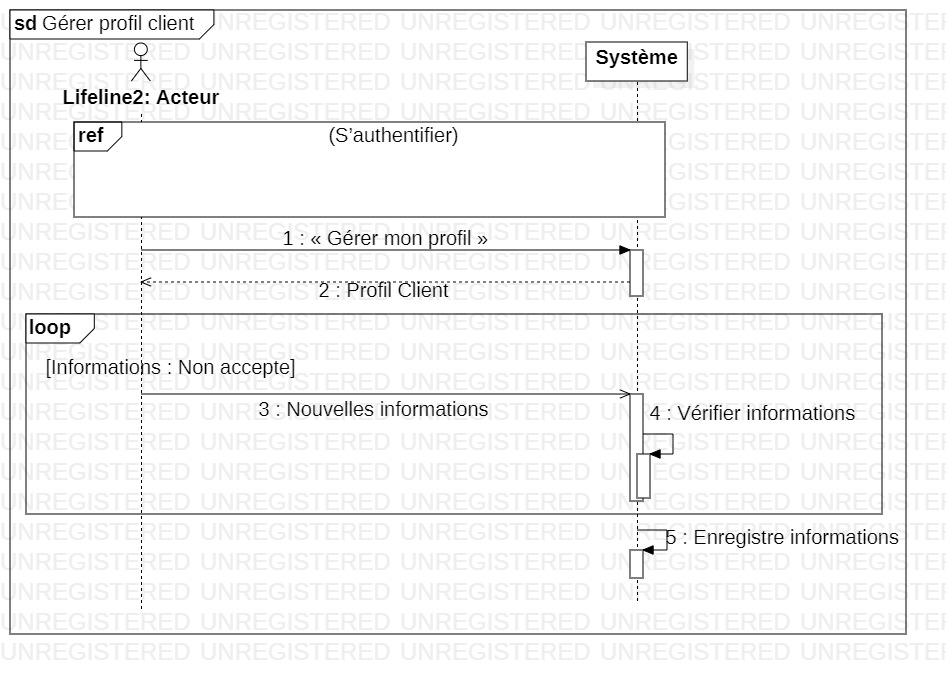
\includegraphics[scale=0.45]{ModifierProfil.jpg}
		\caption{Diagramme séquence Modifier Profil}
		\label{fig:seq update account}
	\end{figure}
\end{center}


\subsection{Cas d'utilisation Poster appel d'offre}
\renewcommand{\arraystretch}{2}
\begin{center}
	\begin{table}[H]
		\centering
		\tiny{\begin{tabular}{ | l | m{0.51\textheight}|}
				\hline
				\rowcolor[HTML]{06a8ed}
				\textbf{Nom du cas} & Poster appel d'offre \\
				\hline \hline
				\cellcolor[HTML]{99ccff} \textbf{Type} & Principal\\
				\hline
				\cellcolor[HTML]{99ccff} \textbf{Acteur Principal} & Client\\
				\hline
				\cellcolor[HTML]{99ccff} \textbf{Objective} & Permet au client de poster un offre de travail pour les artisans\\
				\hline
				\cellcolor[HTML]{99ccff} \textbf{Pré-condition} & S'authentifier\\
				\hline
				\cellcolor[HTML]{99ccff} \textbf{Scénario Nominal} & \parbox{0.43\textheight}{
					\begin{enumerate}
						\vspace{0.01\textheight}
						\item L'acteur clique << Poster appel d'offre >>.
						\item Le site affiche un formualire a remplir.
						\item L'acteur remplis les champs.
						\item L'acteur confirme l'appel.
						\item Le système vérifie informations.
						\item Le système crée un appel d'offre.
						\vspace{0.01\textheight}
				\end{enumerate}}\\
				\hline
				\cellcolor[HTML]{99ccff} \textbf{Scénario Alternatif} & \parbox{0.43\textheight}{
					\begin{enumerate}
						\item \textbf{A1: Les informations du client ne sont pas valides:}
							\subitem 6. Le site affiche message d'erreur.\newline						
						La séquence résume du point 3.
						\item \textbf{A2: Le client annule / ne confirme pas l'appel:}
							\subitem 5. Le site retourne a la page d'acceuile
				\end{enumerate}}\\
				\hline
				\cellcolor[HTML]{99ccff} \textbf{Scénario d'exception} & ---\\
				\hline
				\cellcolor[HTML]{99ccff} \textbf{Post-condition} & Un nouveau appel d'offre sera crée\\
				\hline
		\end{tabular}}
		\caption{Description Poster un appel d'offre}
		\label{table:post appel offre}
	\end{table}
	\begin{figure}[H]
		\centering
		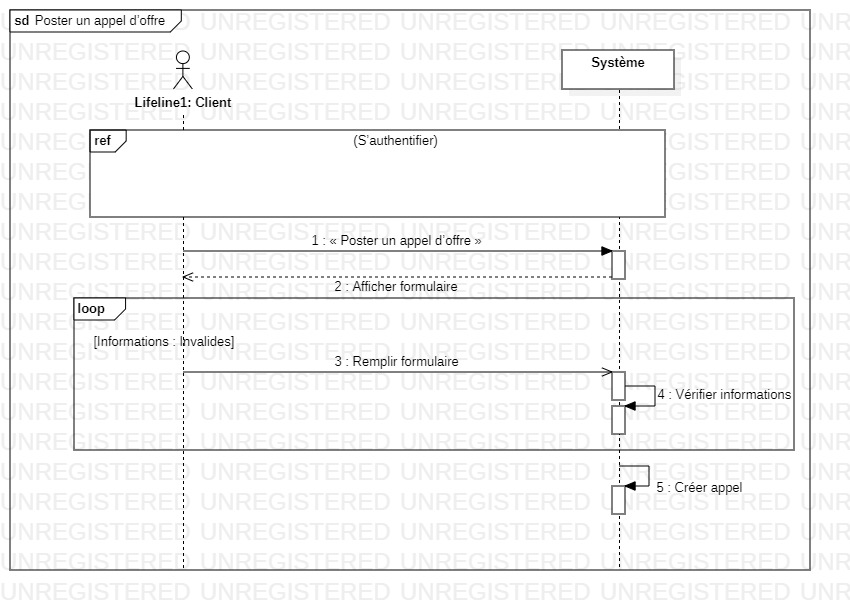
\includegraphics[scale=0.45]{PosterAppelOffre.jpg}
		\caption{Diagramme séquence Poster Appel Offre}
		\label{fig:seq post appel offre}
	\end{figure}
\end{center}


\subsection{Cas d'utilisation Soumission appel d'offre}
\renewcommand{\arraystretch}{2}
\begin{center}
	\begin{table}[H]
		\centering
		\tiny{\begin{tabular}{ | l | m{0.51\textheight}|}
				\hline
				\rowcolor[HTML]{06a8ed}
				\textbf{Nom du cas} & Soumission appel d'offre \\
				\hline\hline
				\cellcolor[HTML]{99ccff} \textbf{Type} & Principal \\
				\hline
				\cellcolor[HTML]{99ccff} \textbf{Acteur Principal} & Artisan\\
				\hline
				\cellcolor[HTML]{99ccff} \textbf{Objective} & Permet à artisan de soumettre un appel d'offre à un client\\
				\hline
				\cellcolor[HTML]{99ccff} \textbf{Pré-condition} & S'authentifier\\
				\hline
				\cellcolor[HTML]{99ccff} \textbf{Scénario Nominal} & \parbox{0.43\textheight}{
					\begin{enumerate}
						\vspace{0.01\textheight}
						\item Artisan cliquer sur << Soumettre appel d’offre >>
						\item Le système affiche la liste des offres
						\item L'artisan soumis un ou plusieurs offres
						\item Le système sauvegarde la soumission
						\item Le système notifie le client
						\vspace{0.01\textheight}
				\end{enumerate}}\\
				\hline
				\cellcolor[HTML]{99ccff} \textbf{Scénario Alternatif} & --- \\
				\hline
				\cellcolor[HTML]{99ccff} \textbf{Scénario d'exception} & --- \\
				\hline
				\cellcolor[HTML]{99ccff} \textbf{Post-condition} & Un appel d'offre sera soumis\\
				\hline
		\end{tabular}}
		\caption{Description Soumission d'un appel d'offre}
		\label{table:soumettre offre}
	\end{table}
	\begin{figure}[H]
		\centering
		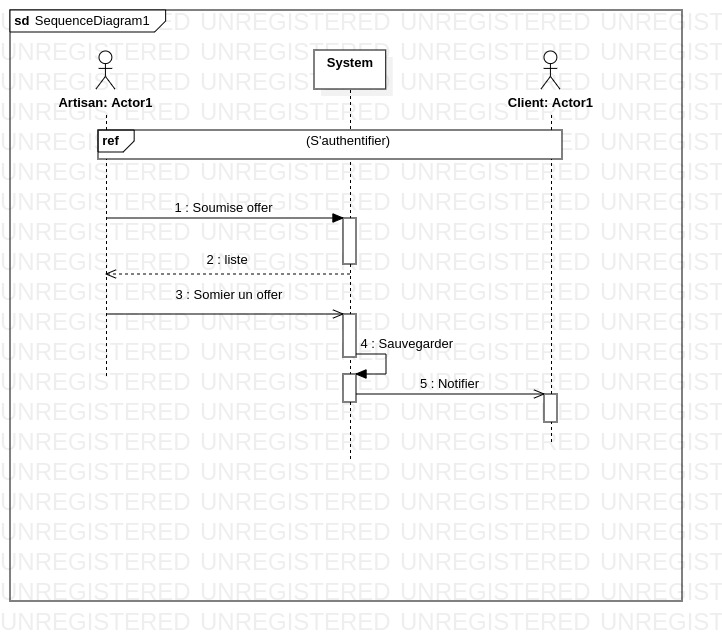
\includegraphics[scale=0.45]{SoumttreOffre.jpg}
		\caption{Diagramme séquence Soumettre un appel d'offre}
		\label{fig:seq soumettre offre}
	\end{figure}
\end{center}


\subsection{Cas d'utilisation Signaler un utilisateur}
\renewcommand{\arraystretch}{2}
\begin{center}
	\begin{table}[H]
		\centering
		\tiny{\begin{tabular}{ | l | m{0.51\textheight}|}
				\hline
				\rowcolor[HTML]{06a8ed}
				\textbf{Nom du cas} & Signaler un utilisateur \\
				\hline\hline
				\cellcolor[HTML]{99ccff} \textbf{Type} & Principal \\
				\hline
				\cellcolor[HTML]{99ccff} \textbf{Acteur Principal} & Client, Artisan\\
				\hline
				\cellcolor[HTML]{99ccff} \textbf{Objective} & Permet à un utilisateur de signaler un autre utilisateur\\
				\hline
				\cellcolor[HTML]{99ccff} \textbf{Pré-condition} & Consulter Profil\\
				\hline
				\cellcolor[HTML]{99ccff} \textbf{Scénario Nominal} & \parbox{0.43\textheight}{
					\begin{enumerate}
						\vspace{0.01\textheight}
						\item L'acteur clique consulte le profil de l'utilisateur.
						\item Le site affiche le profil de l'utilisateur.
						\item L'acteur clique sur << Signaler >>.
						\item Le système affiche un forumalire a remplir.
						\item L'acteur remplis le formulaire.
						\item Le système vérifie informations.
						\item Le système envoie sauvgarde le rapport et l'envoie aux administrateurs.
						\vspace{0.01\textheight}
				\end{enumerate}}\\
				\hline
				\cellcolor[HTML]{99ccff} \textbf{Scénario Alternatif} & \parbox{0.43\textheight}{
					\begin{enumerate}
						\item \textbf{A1: Les informations du formulaire ne sont pas valides:}
						\subitem 7. Le site affiche message d'erreur.\newline						
						La séquence résume du point 4.
						\item \textbf{A2: Le client annule / ne confirme pas l'appel:}
						\subitem 5. Le site retourne a la page d'acceuile
				\end{enumerate}}\\
				\hline
				\cellcolor[HTML]{99ccff} \textbf{Scénario d'exception} & --- \\
				\hline
				\cellcolor[HTML]{99ccff} \textbf{Post-condition} & Un rapport sera envoyé aux administrateurs\\
				\hline
		\end{tabular}}
		\caption{Description Signaler un utilisateur}
		\label{table:signaler utilisateur}
	\end{table}
	\begin{figure}[H]
		\centering
		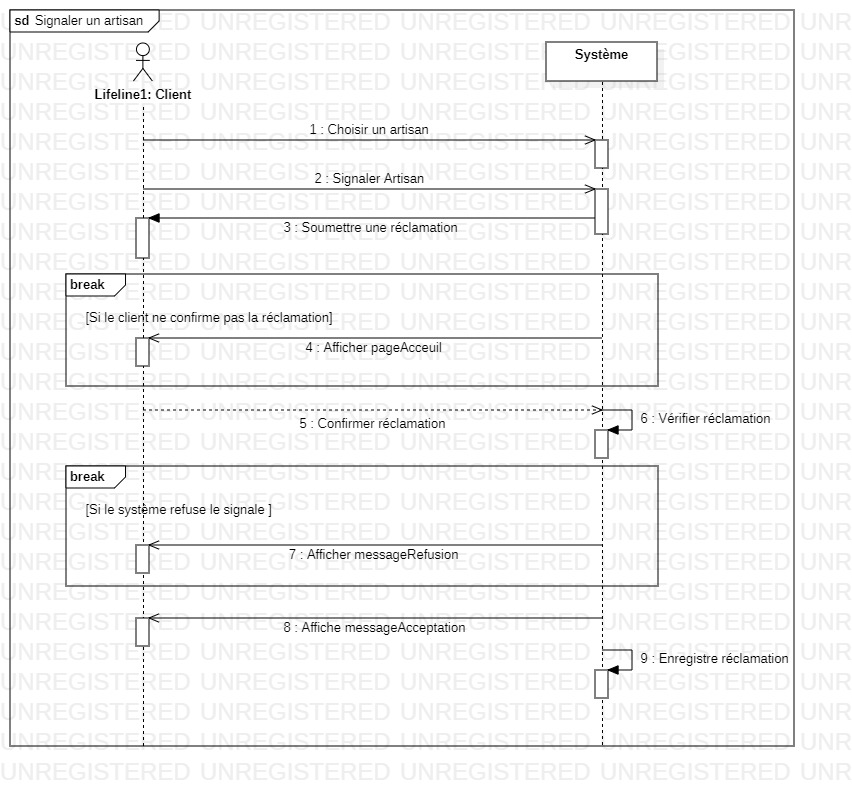
\includegraphics[scale=0.44]{SignalerUtilisateur.jpg}
		\caption{Diagramme séquence Signaler un Utilisateur}
		\label{fig:seq signaler utilisateur}
	\end{figure}
\end{center}


\subsection{Cas d'utilisation Bloquer un utilisateur}
\renewcommand{\arraystretch}{2}
\begin{center}
	\begin{table}[H]
		\centering
		\tiny{\begin{tabular}{ | l | m{0.51\textheight}|}
				\hline
				\rowcolor[HTML]{06a8ed}
				\textbf{Nom du cas} & Bloquer un utilisateur \\
				\hline\hline
				\cellcolor[HTML]{99ccff} \textbf{Type} & Principal \\
				\hline
				\cellcolor[HTML]{99ccff} \textbf{Acteur Principal} & Administrateur\\
				\hline
				\cellcolor[HTML]{99ccff} \textbf{Objective} & Permet à un administrateur de bloquer (banner) un utilisateur\\
				\hline
				\cellcolor[HTML]{99ccff} \textbf{Pré-condition} & S'authentifier\\
				\hline
				\cellcolor[HTML]{99ccff} \textbf{Scénario Nominal} & \parbox{0.43\textheight}{
					\begin{enumerate}
						\vspace{0.01\textheight}
						    \item L’acteur visite la fenêtre d’édition
							\item Une liste de tous les utilisateurs sera affichée
							\item L’administrateur clique sur l’utilisateur voulu
							\item L’admin clique sur bouton bloquer
							\item Un message confirmation s’affichera
							\item L’admin confirme son action
							\item Le systeme banne l'utilisateur
						\vspace{0.01\textheight}
				\end{enumerate}}\\
				\hline
				\cellcolor[HTML]{99ccff} \textbf{Scénario Alternatif} & \parbox{0.43\textheight}{
					\begin{enumerate}
						\item \textbf{A1: L'administrateur annule l'action:}
						\subitem 7. Le systeme affiche la page d'acceuille.\newline						
						\item \textbf{A2: L'utilisateur est un autre administrateur:}
						\subitem 7. Le systeme affiche un message d'erreur.
						\subitem 8. Le systeme affiche la page d'acceuille.
				\end{enumerate}}\\
				\hline
				\cellcolor[HTML]{99ccff} \textbf{Scénario d'exception} & --- \\
				\hline
				\cellcolor[HTML]{99ccff} \textbf{Post-condition} & L'utilisateur sera banné\\
				\hline
		\end{tabular}}
		\caption{Description Bloquer un utilisateur}
		\label{table:bloquer utilisateur}
	\end{table}
	\begin{figure}[H]
		\centering
		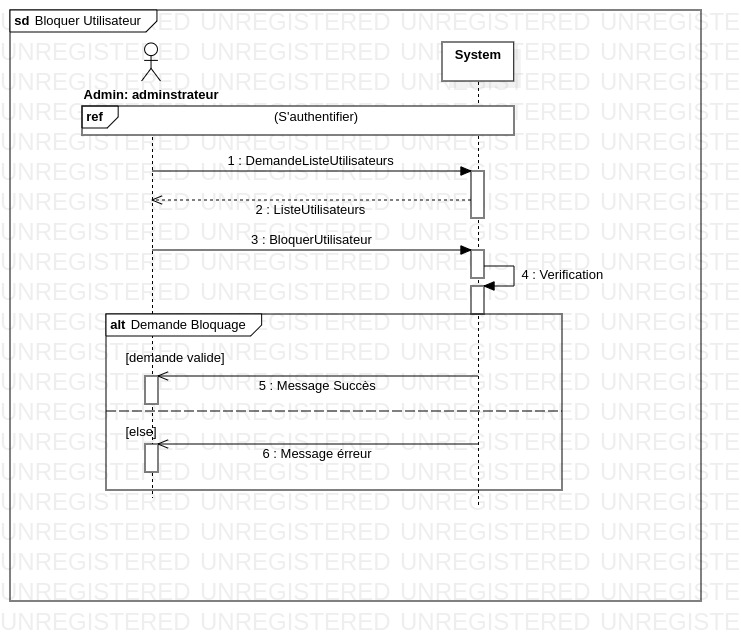
\includegraphics[scale=0.52]{BloquerUtilisateur.jpg}
		\caption{Diagramme séquence Bloquer un Utilisateur}
		\label{fig:seq bloquer utilisateur}
	\end{figure}
\end{center}


\subsection{Cas d'utilisation Gérer réclamations et signalements}
\renewcommand{\arraystretch}{2}
\begin{center}
	\begin{table}[H]
		\centering
		\tiny{\begin{tabular}{ | l | m{0.51\textheight}|}
				\hline
				\rowcolor[HTML]{06a8ed}
				\textbf{Nom du cas} & Gérer réclamations et signalements \\
				\hline\hline
				\cellcolor[HTML]{99ccff} \textbf{Type} & Principal \\
				\hline
				\cellcolor[HTML]{99ccff} \textbf{Acteur Principal} & Administrateur\\
				\hline
				\cellcolor[HTML]{99ccff} \textbf{Objective} & Permet à un administrateur de Gérer une réclamations et de prendre une action\\
				\hline
				\cellcolor[HTML]{99ccff} \textbf{Pré-condition} & S'authentifier\\
				\hline
				\cellcolor[HTML]{99ccff} \textbf{Scénario Nominal} & \parbox{0.43\textheight}{
					\begin{enumerate}
						\vspace{0.01\textheight}
						\item L’acteur visite la fenêtre des réclamations et signalements
						\item Une liste de tous les réclamations et signalements s’affiche
						\item L’administrateur clique sur une réclamation / signalement
						\item Détailles de la réclamation / signalement s’affiche
						\item L’administrateur, après avoir lu la réclamation, peut soit, en cliquant sur un bouton, l’accepter, la refuser ou contacter la source du réclamation pour plus de détails
						\item En cas d’accepter la réclamation, l’admin sera redirigé vers une nouvelle page (gérer compte utilisateur) pour choisir une action  
						\vspace{0.01\textheight}
				\end{enumerate}}\\
				\hline
				\cellcolor[HTML]{99ccff} \textbf{Scénario Alternatif} & --- \\
				\hline
				\cellcolor[HTML]{99ccff} \textbf{Scénario d'exception} & --- \\
				\hline
				\cellcolor[HTML]{99ccff} \textbf{Post-condition} & La réclamation sera résolu\\
				\hline
		\end{tabular}}
		\caption{Description Gérer réclamations et signalements}
		\label{table:gerer reclamation}
	\end{table}
	\begin{figure}[H]
		\centering
		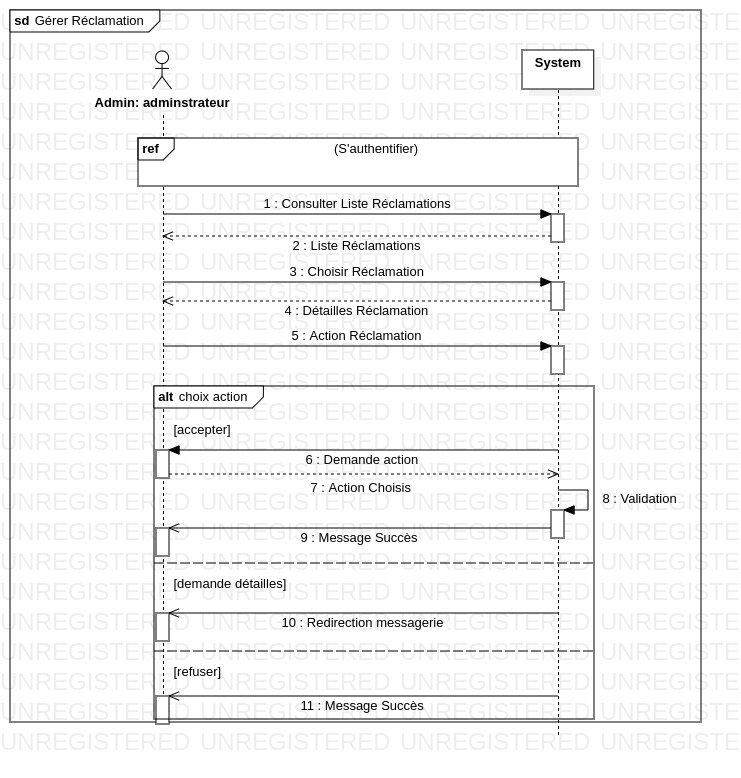
\includegraphics[scale=0.45]{GererReclamation.jpg}
		\caption{Diagramme séquence Gérer réclamations et signalements}
		\label{fig:seq gere reclamation}
	\end{figure}
\end{center}

\section{Conclusion}
Dans ce chapitre, nous avons présenté l’analyse des besoins dont on identifient les acteurs / utilisateurs qui interagissent avec notre future application suivi par la spécification des besoins fonctionnels et techniques(non-fonctionnels), modélisés sous forme des diagrammes.\\

On finalise par la description détaillée et les diagrammes de séquences des cas dont on a jugé important ou intéressant.

\vspace{0.01\textheight}
On se basant sur les descriptions et diagrammes précédents, on entame le deuxième chapitre du conception
